\documentclass[runningheads]{llncs}

\usepackage[T1]{fontenc}
\usepackage{graphicx}
\usepackage{comment}

\begin{document}

\title{PErsoNal Genome QUery IN healthcare and clinical practice (PENGQUIN)}

\author{Elias Crum\inst{1,2}\orcidID{0009-0005-3991-754X}}

\authorrunning{E. Crum}
\institute{IDLab, Department of Electronics and Information Systems, Ghent University - imec \and Flemish institute for Technological Research (VITO)}


\maketitle

\begin{abstract}
    Medical care is in the process of becoming increasingly personalized through the use of patient genetic information. 
    At present, data useful for clinical care, including genetic data, is commonly diffuse, organized arbitrarily, and stored in data silos. 
    Thus, unstructured organization, high costs for data storage and generation, and tight privacy restrictions pose serious challenges to scaling personalized clinical strategies.
    I propose an early stage Ph.D. that aims to improve the connectedness and shareability of genomic data storage(s), while preserving data privacy, to decrease the costs of using patient genome data in clinical practice. 
    In this pursuit, I will integrate various domains of semantic web research into a novel, holistic framework designed for use in clinical practice.
    Specifically, I will (a) store patient data using Solid pods, (b) represent personal genome sequence data in RDF as Linked Data, (c) attach policies to stored data, and (d) query data through link traversal queries.

\keywords{Solid \and Linked Data \and Querying \and Genomic Data Sharing}

\end{abstract}


\section{Introduction / Motivation}
As our understanding of genomics deepens, the role of Personal Genome Sequencing (PGS) in healthcare is expanding. 
At the time of writing, there are multiple domains of clinical practice where patient PGS data is now used to inform medical decision making, including drug development \cite{ko_new_2022}, cancer diagnosis and treatment \cite{mcleod_cancer_2013}, and rare genetic disease identification and treatment \cite{marwaha_guide_2022}.
How this integration is deployed varies by clinical domain, but improved outcomes have generally been observed \cite{mathur_personalized_2017}.
Despite great promise, barriers to adoption remain \cite{stefanicka-wojtas_barriers_2023}. 
One major challenge is presented by the digital representation, storage, and access to the PGS data that underlies clinical usage.
With my Ph.D., I aim to address the challenges presented by PGS data usage in clinical practice by leveraging decentralized storage, data representation, and querying technologies.

\textbf{PGS data storage and sharing.} 
PGS data are expensive to both generate and store. 
The average human genome is slightly over 3 billion base pairs in length (3 Gbp). 
During a whole genome sequencing workflow, various sequence formats that offer different sets of information are produced \cite{bagger_whole_2024}.
Of these, Variant Call Format (VCF) files \cite{danecek_variant_2011} serve as the state-of-the-art for most clinical genomic applications.
VCF files are typically between 100-1000s MBs within computer memory and represent around 3 million nucleotide positions of an individual\textquotesingle s PGS.
For these genomic data, there are also significant privacy considerations.
Unfortunately, the relationship between privacy and cost is largely antagonistic within the current technological framework.
Increases in privacy protections often lead to increases in data siloing and increased costs for both patient and provider.
For instance, if a patient moves hospitals, it is common for PGS data and genomic tests to be regenerated and indefinitely stored in that new location because of the lack of data sharing between institutions.
One strategy for reducing costs is through increased data sharing and data discoverability between hospital systems.
Another increase in efficiency could be achieved by greater connectivity of a single patient\textquotesingle s data, such as previous test results, PGS data, medical history, etc.
Increasing patient data connectedness and accessibility for authorized users is not a trivial problem while also maintaining privacy.
It is at this crossroads that the current state-of-the-art in clinical data storage technology is largely incapable of achieving both goals.

\textbf{A Solid solution.} 
A possible solution to the challenges faced is through reorganization of how data is stored and discovered. 
The citizen-centric model places the patient at the center and is not an entirely novel concept \cite{brands_patient-centered_2022}.
Within the current system, a citizen-centric model is difficult to implement due to technological challenges presented by centralized databases.
The Solid protocol \cite{capadisli_solid_nodate}, a decentralized data storage approach, is composed of specifications more conducive to construction of a citizen-centric data storage strategy for clinical data.
Specifically, Solid offers the ability to granularize data privacy, allow authorized data access over the web, and represent stored data as Linked Data, all features that can work to remove some of the antagonism between cost reduction and privacy preservation.

\textbf{Project motivation.}
Despite there being no real solutions to the current antagonism between privacy and cost reduction for PGS data usage in healthcare, there is also a conspicuous gap in the current scientific discourse around the development and implementation of a proposed solution. 
This gap underscores the necessity of my Ph.D.
I aim to improve the connectedness and shareability of genomic data storage(s) while preserving data privacy, through the integration of various domains of semantic web research into a novel, holistic framework designed for use in clinical practice. 
My Ph.D. will also aim to demonstrate the limitations of current state-of-the-art semantic web technologies in this novel application domain with the intention of driving innovation and discovering future research pursuits.


\section{State of the Art}
\begin{comment}
Describe existing work in the area, work focusing on the same/similar problems or that might be useful to tackling your research question.
\end{comment}

\textbf{Current clinical data storage.}
Most clinically relevant health data, including PGS data, is stored using an institution-centric approach characterized by the hospital or hospital system isolating its stored data into one or more centralized or cloud-based databases that are governed and maintained solely by the owner institution or a contracted organization \cite{quantin_medical_2011}. 
The predominant organization of these databases is a relational structure, although alternative non-relational methods like NoSQL or RDF have become slightly more popular in recent years \cite{kotsilieris_efficient_2021}.
Due to technological limitations imposed by relational database structure, maintaining stored data privacy results in strict data accessibility policies that severely restrict data sharing potential.
With the enlarged threat of hacking, phishing, and login credential compromisation that is only increasing \cite{noauthor_ransomware_nodate}, health care institutions have taken steps to enact tighter restrictions on data access and increase cyber security budgets.  
Collectively, these state-of-the-art approaches to PGS data storage inhibit the scalability of PGS data usage in clinical practice due to data siloing and resulting high costs.

\textbf{PGS data sharing in academic research.}
In academic research, the development of infrastructure that allows for sharing of genome data between institutions, creating federated centralized databases, can be observed in initiatives such as GA4GH Beacons \cite{rambla_beacon_2022}.
Despite this step towards increased sharing and cost reduction, advancements in state-of-the-art infrastructure and standards are not directly translatable to clinical practice. 

\textbf{Solid, RDF, and Linked Data in clinical practice.}
The Solid specifications have been shown to provide competent infrastructure for preserving the privacy of sensitive stored data \cite{esposito_assessing_2022}.
Further, it has been shown that additional safeguards can be imposed using privacy policies represented in RDF triples, allowing more granular discoverability controls \cite{benaribi_sparql-based_2023}. 

In recent years, there have been initiatives for representing biological data as RDF \cite{sib_swiss_institute_of_bioinformatics_rdf_group_members_sib_2024}, specifically extending into clinical biology recently \cite{van_der_horst_bridging_2023}. 
Past experiments have shown that general linked data integration into clinical practice results in improved outcomes \cite{farinelli_linked_2015}.
There is also precedent for investigation into the representation of genomic information as RDF \cite{prasanna_scalable_2023}\cite{van_der_horst_bridging_2023}.
Solid pods could provide the infrastructure for such data storage strategies, while also preserving possibilities for non-linked data stored in the pod, such as test result files, to be linked to genomic data, improving data connectivity. 

\textbf{Link Traversal Query Processing (LTQP).}
To make sense of linked genomic and clinical data approaches to parsing and querying that data must also be investigated, especially to encourage greater data discoverability and usage in clinical practice.
Recent work has established that the querying of Linked Data in decentralized environments is possible \cite{taelman_evaluation_2023}, but these results were obtained with assumptions different than those presented by patient genome pods.
Here, querying will be performed over a potentially large number of data pods containing large amounts of linked data, a situation not extensively investigated. 

\section{Problem Statement and Contributions}
\begin{comment}
Formulate the problem you intend to solve, and how you intend to contribute to Semantic Web research. This section should include a clear formulation of one (or very few) research hypothesis (what statement you want to validate through your methodology, approach and evaluation), and/or the research questions that need to be answered.
\end{comment}

My Ph.D. is situated to provide a proof-of-concept PGS data storage and querying framework for use in clinical practice. 
In this pursuit, my core research question is: 
\textit{Can combining the Solid specifications for data storage with other compatable cutting-edge innovations in data policy, linking, and querying be instantiated and deployed as a framework that provides advantages over the existing PGS data storage protocols in health care?}

To address this central question, I will investigate the more specific questions: 
A) Can the decentralized storage protocol Solid \cite{capadisli_solid_nodate} offer suitable infrastructure for PGS data? 
B) Do the specifications provided by Solid provide for adequate control of PGS data privacy while also allowing for increased authorized sharability? 
C) Can querying over these sources be achieved through the use of modified LTQP algorithms?
D) Can these features be combined into a cohesive web application and deployed together?

My hypothesis is that such a framework can be developed and would offer unique advantages over the existing state-of-the-art institution-centric PGS data storage solutions. 

The following five objectives will be undertaken to test my hypotheses:
(1) Solid Pod PGS Data Storage, 
(2) Genomic data as Linked Data,
(3) Data policies,
(4) Data querying,
(5) Framework deployment.

Together, these objectives will serve as the components of an operational framework. 
The framework, once produced, will be compared to existing strategies for storing and sharing PGS data to assess the efficacy of transitioning toward product production and specific clinical use case adaptation.
The proposed scientific approach also aims to test the application of numerous fields of semantic web research to a clinical knowledge domain. 
Explicitly, an approach to how decentralized storage specifications can be applied to sensitive medical data storage, how genomic and medical data can be represented and queried as Linked Data, how existing Linked Data querying algorithms perform over genomic and health data, how granularized data policies impact querying and linking data in a medical context, and how the combination of these semantic technologies could provide an improvement over existing state-of-the-art clinical PGS data storage and usage strategies, are specific questions my Ph.D. aims to answer.


\section{Research Methodology and Approach}
\begin{comment}
Describe the research methodology you will apply in your research, including the different steps from the formulation of your research questions to answering them. Also describe the approach you are taking (or you intend to take for Early Stage Ph.D. submissions) to instantiate the research methodology, hence contributing to solve the problem described in Section 3 and confirm or reject your hypothesis. Discuss how this approach is innovative and novel, and how it is (might be) implemented.
\end{comment}

My Ph.D. will be split into four component work packages (WPs) with a fifth work package where the components will be unified into a cohesive framework with an accompanying web application. This workflow is reflected in Fig. 1.

\begin{figure}
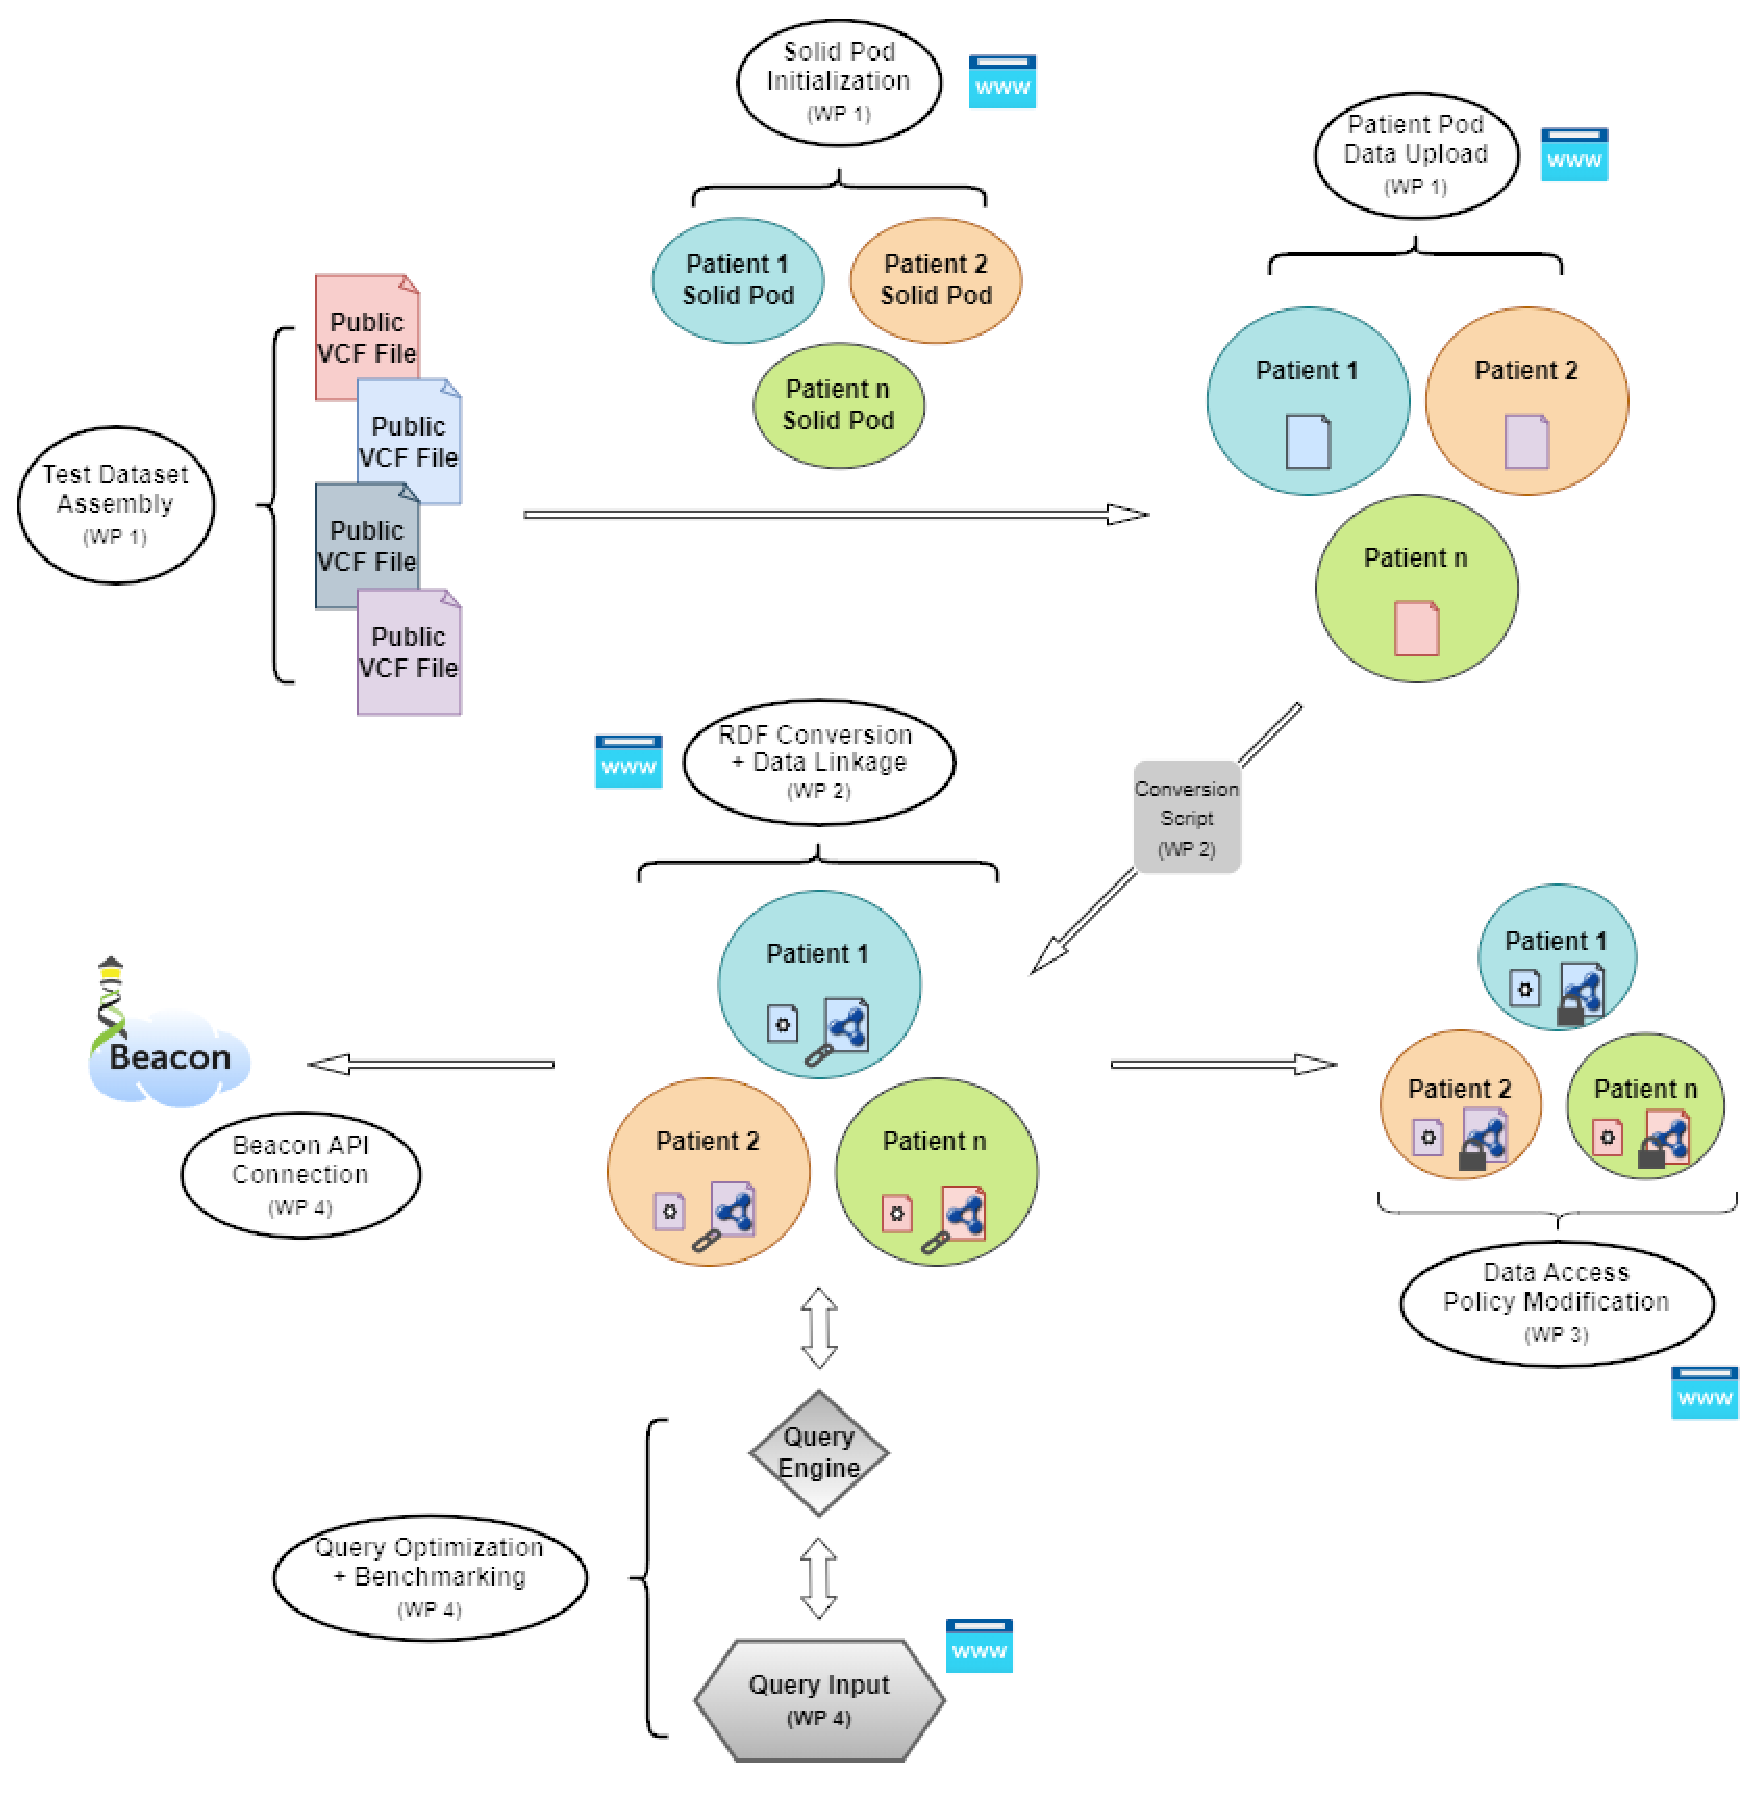
\includegraphics[width=\textwidth]{fig1.eps}
\caption{\textbf{PENGQUIN Ph.D. workflow.}
White circles represent milestones to be achieved in respective work packages (WP) that are denoted in parentheses. 
The small blue "WWW" box seen next to some objectives represents integration of that item into the framework\textquotesingle s web application.
WP 1 will achieve the assembly of a VCF file test dataset, the initialization of simulation Patient Solid Pods, and the upload of simulation patient VCF files into that patient's Solid pod.
WP 2 will convert VCF file data into a serialized RDF representation and link parts of that VCF data to other simulated medical data.
WP 3 will establish data access policies for patient Solid pods and specific data stored within them.
WP 4 will experiment with querying approaches for discovering and accessing data stored in patient Solid pods through the use of user provided queries and the use of a query engine.
WP 5 will establish the connection of the patient's Solid pod to the Beacon network.
} \label{fig1}
\end{figure}

\begin{comment}
1. Research question --> how to answer
2. how do you plan to test hypothesis
3. how is the approach novel / how it is implemented
\end{comment}

\subsection{Work Package 1: Storing and publishing personal genomic data in a decentralized environment} 

I will test the viability of Solid data pods as storage infrastructure for patient PGS data, thus, testing my hypothesis that Solid can support PGS data storage. 

A test dataset will be constructed using publicly available Illumina platinum genome files \cite{noauthor_platinum_nodate}. 
These files will be used as representative "patient" PGS data for experimentation. 

I will also create server-hosted Solid pods using the Community Solid Server (CSS) implementation of Solid \cite{css}. 
Each pod will be a storage container for a single individual\textquotesingle s PGS data. 
I will upload a single VCF file, into one "patient\textquotesingle s" pod to test basic functionality of a Solid pod for hosting large patient genomic data. 
The use of the CSS for Solid pod hosting for research purposes is state-of-the-art, but there have been no published experiments documenting the use of Solid pods for storing PGS data, which are much larger than the datasets used in past Solid experimentation. 
The main risk of storing PGS data in Solid data vaults is related to the size of PGS data which will be addressed through organizational large-scale storage access. 


\subsection{Work Package 2:  Storing PGS data in RDF and as Linked Data}

I hypothesize that the conversion from VCF to RDF is possible, and the resulting RDF representation will allow for linking of other medically relevant data within the patient\textquotesingle s pod and outside of it.
The conversion process will be made reversible to enable connection to existing clinical workflows that request VCF format. 

To convert PGS data from VCF to RDF, we will investigate a format translation process using the SPHN RDF ontology \cite{van_der_horst_bridging_2023}. 
During this translation process, we will experiment with different approaches, such as a bidirectional mapping index, for efficient reversal of conversion.

I then intend to demonstrate the linking of part of a patient\textquotesingle s genome to
(A) other data within the patient\textquotesingle s pod, 
(B) data in a public database outside of a patient\textquotesingle s pod, and
(C) data from another patient\textquotesingle s pod.
Linkages will be added through triple insertions at different relevant points in the serialized VCF RDF file stored in the patient's Solid Pod.
All data linkages will be made using files and triples that contain simulated data or publicly available data.

While Linked Data is state-of-the-art, these concepts have not yet been applied to clinical genomic data.
The power of linking the VCF data to other clinically relevant data will be especially realized when these semantic links are discovered during querying, which will be investigated in WP5. 

The main risk of converting PGS data to Linked Data using RDF is that this conversion requires an ontology. 
The conversion process will utilize the publicly available SPHN RDF ontology~\cite{van_der_horst_bridging_2023} and if this ontology is insufficient, I will work with members of the IDLab at UGhent with experience in ontology definition to make changes or additions where necessary.


\subsection{Work Package 3: PGS data privacy policies}

In this work package, I will experiment with the design and implementation of multiple levels of authorization as well as methods that allow for dynamic control over data discoverability, read/write access, and data access consent requests within a patient\textquotesingle s Solid pod. 
I hypothesize that various levels of authorization can be implemented and provide protections for maintaining the privacy of PGS data stored in Solid pods.

I will develop and test three functionalities for privacy modifications.
(1) registration of a pod to an individual patient,
(2) submission of a request to access stored data from a data requester, the notification of the patient, and the consent or denial by the patient, and
(3) permission revoking capabilities as well as an opt-in option to share their data with researchers. 
All of these methods will be integrated into the framework\textquotesingle s web application.
To utilize these methods, various levels of access to pod read and write privileges will be created and filled to represent a real clinical PGS workflow. 

Assigning the above permissions within Solid is an open area of research and there are currently state-of-the-art protocols implemented in the CSS that allow their implementation.
The described access schema has not been attempted in the presented level of detail for clinical genomic data.
If the above proposed schema for privacy policies cannot be achieved, a simpler and more generalized schema will be devised and implemented.
Privacy is a nuanced subject, especially in terms of governance and here, I aim to show the possibilities presented by Solid in this framework, not dictate suggestions for its deployable implementations. 

\subsection{Work Package 4: Querying over PGS data in one and many pods}

This work package will establish a querying mechanism for patient pod data that incorporates user permissions and data linkages. 
I hypothesize that a querying functionality that utilizes a query engine computational strategy will be able to query over patient Solid pods and return query results.

I will execute queries across PGS data contained in patient pod(s) through the use of the query language SPARQL \cite{noauthor_sparql_nodate}.
Query execution requires a source for computation which is not currently provided by the Solid pods themselves.
I will investigate the use of a query engine, such as that offered by Comunica \cite{comunica}, to perform the queries apart from the data stores.

For PGS data querying, I will benchmark and build upon the link traversal query processing (LTQP) paradigm \cite{taelman_evaluation_2023}, which has been shown to be an effective method for querying Linked Data between Solid Pods. 
A significant challenge is presented by the storage landscape of a large number of large data sources.
I will look to innovate established LTQP algorithmic approaches by integrating strategies that leverage the unique structure of PGS data such as the use of pre-computed indexes, like the one generated for RDF-VCF conversion, as a guide for faster query processing.

I aim to adapt this querying approach to the specific domain of genomic and health data which has not been attempted before. 
There is a risk that I cannot devise solutions to incorporating indexes in LTQP algorithms and/or these algorithm modifications do not improve performance enough to be usable.
If these challenges are encountered, I will first investigate imposing limits on query complexity and reducing the number of data vaults that are included in the possible query space, then, if still unsuccessful, look to investigate the implementation of algorithms utilized by centralized SPARQL endpoints that are known to be able to query large sets of data. 


\subsection{Work Package 5: Component consolidation and framework deployment}

To improve data flows for research purposes, I intend to connect the proposed framework to the international Beacon initiative \cite{rambla_beacon_2022}. 
In this aim, I will investigate the establishment of patient Solid pods, containing PGS data, as beacon endpoints that can be discoverable and queried via the Beacon API. 
The connection of a decentralized, citizen-centric storage framework to the Beacon network is novel in nature as all other existing endpoints are institution-centric relational databases maintained by hospitals or research institutions.
Any issues within this aim will be addressed through collaboration with creators of the Beacon initiative.

All other functionalities will also be packaged into a web application with supporting documentation for final deployment and exhibition of how such a framework could function in clinical practice.
This framework would be the first of its kind.


\section{Evaluation Plan}
\begin{comment}
Describe your evaluation or evaluation plan, which is the way you (intend to) validate your hypothesis, your results, and the value of your approach.
\end{comment}

\textbf{WP1}.
All tasks within WP1, including test dataset assembly, Solid pod creation and hosting using the CSS, and test data uploading to Solid pods will be evaluated only for functionality.

\textbf{WP2}.
Direct conversion between VCF and RDF will be evaluated in terms of computational overhead, conversion time, and memory usage, both in the Solid pod and during conversion.
The same evaluations will also be performed on the process when an intermediate mapping index file is used. 
Comparisons will be documented in a formal benchmarking study.
Functionality of data linkage aims will be assessed by data querying in WP4.

\textbf{WP3}
Attaching differing levels of authorization to data will be assessed by creating various profiles that reflect clinical roles and access levels and attempting to access data via user-mediated, application requesting, and querying approaches. 

\textbf{WP4}
Query engine functionality will be evaluated using query execution time and computational load metrics as well as query results assessment. 
Query results will establish the functionality of data linkages from WP2.
Benchmarking will be done for existing LTQP algorithms and altered query algorithms that utilize genomic index files and results will be compared.
Ideally, success will be determined by queries that return correct results in under 10 minutes for users and potentially longer for applications.
In a clinical setting, time constraints are not as important as accuracy and reliability of results, although excessive query times decrease the usefulness of such a tool for physicians in clinical practice.

\textbf{WP5}
Beacon API connection will be evaluated on functionality and integrate all previous work package components. 
Similarly, evaluation of the web application from which a user can interact with the framework will also be based on functionality.


\section{Preliminary Results}
\begin{comment}
Results: Report the results achieved up to now in applying your approach in this section. Preliminary results are fine.
\end{comment}

During the first months of my Ph.D., I have been composing a scoping review paper on the current landscape of clinical genomic data sharing.
I plan to submit the review paper for publication in a peer-reviewed journal in the coming months.
Within WP1, I have successfully assembled the test dataset and set up CSS pod instances.
I have also successfully uploaded VCF files into these pods signalling completion of WP1. 


\section{Conclusions/Lessons Learned}
\begin{comment}
Present your conclusions and lessons learned. Describe how your results will or might impact research or the world at large. We do neither expect you to have solved all issues nor expect you to have finished your Ph.D. However, we expect you to show an understanding of your research area in general and to have a clear plan towards addressing your research questions. This symposium is the best place to discuss these issues and plans with experienced researchers and fellow students to get informed feedback.
\end{comment}

With the emergence of patient genomic data as a tool for clinicians, establishing the infrastructure for patient genomic data sharing that maintains patient data privacy is an economic niche that is largely unfilled. 
My Ph.D. framework is poised to provide the outline of necessary technological implementation considerations while hopefully contributing to future product development. 
More generally, my Ph.D. is designed to assess the potential in applying cutting-edge semantic web research to modern clinical challenges with the hope of gaining insight into the efficacy of these applied implementations while identifying future research directions.



\subsubsection{\ackname} 
I acknowledge my Ph.D. promoters Ruben Taelman\inst{1}, Bart Buelens\inst{2}, Gokhan Ertaylan\inst{2}, and Ruben Verborgh\inst{1} for their help and guidence.
Funding provided from VITO NV (\verb|UG_PhD_2303_contract|). 

\bibliographystyle{splncs04}
\bibliography{ESWC_Project_Description_EDC}

\end{document}
